%-------------------------------------------------------------------------------
\hypertarget{lcap6}{}
\chapter{Conclusions}
\vspace{-1cm} \label{cap6} 
%\begin{flushright}
%\begin{minipage}{0.7\linewidth}
%\emph{``Enquanto existir vontade de lutar, existem esperan�as de
%vencer.''}
%\end{minipage}
%\end{flushright}
%
%\begin{flushright}
%{A. Agostinho}
%\end{flushright}


\section{Project Overview}

In this study, we investigate how neglecting timestamps of irregularly sampled measurements may affect state estimation performance, under different conditions. 

The research motivations are discussed in Chapters \ref{cap2} and \ref{cap3}, where sensor fusion methods and irregular sampling schemes are reviewed, respectively. We note how sensor fusion, as a field of science, has been experiencing significant growth due to cheaper sensors and communication devices. Bigger and more complex sensor networks are more and more common, and so are the related challenges, such as irregular sampling. Then we define the irregular sampling problem and review the main schemes studied in the literature. Timestamps are often needed in order to take these irregularities into account in data fusion processes. We note that sometimes due to computational complexity or the need of investment in time synchronization techniques, such assumption is not always guaranteed. Thus we conclude the literature review focusing in the study of sensor fusion applied to state estimation and how it is affected when timestamp is neglected.

In Chapter~\ref{cap4} we describe the algorithms used in the numerical simulations. We begin by describing the discrete-time representation of sampled-data systems, considering variable time steps in the discretization process, since measurements are sampled aperiodically. We also review the most popular state estimation algorithm, that is the Kalman Filter (KF), and one of its variation for nonlinear cases, the unscented Kalman Filter (UKF). We describe them as a data fusion process, using the Bayesian framework. Then we describe the sampling irregularity model, which is considered to be given by a Poisson process, meaning that the waiting time between two consecutive measurements is a exponential random variable (RV). Moreover, we describe the adaptations made to the algorithms due to the aperiodic sampled measurements. Whenever timestamps are not available, the measurements are considered to be taken in the next regular estimation interval. A first glimpse of the added error introduced by neglecting timestamps is also presented in this chapter. We end it by defining performance metrics used in the simulation, that cover both accuracy and consistency.

Numerical results are presented in Chapter~\ref{cap5}. We begin by studying the error effects on measurements introduced by shifting the time instants they were taken, and how these errors are related to signal-to-noise ratios (SNR) and system dynamics. Based on that, we propose a simulation setup, where system parameters are varied to assess their relation to state estimation performance, knowingly: (i) measurement noise levels, or SNR; (ii) average sampling rate of measurements, referred to as $\lambda$; and (iii) the relation between $\lambda$ and the regular sampling rate of the estimation, referred to as $\alpha$. Two systems are chosen as case studies: a fourth-order linear time invariant system; and a nonlinear system given by a nonholomonic moving unicycle robot, whose position in the $xy$-plane must be estimated. We illustrate the state estimation problem under irregular sampling by one realization of the estimates. To assess the performance differences from the algorithms that consider and neglect measurement timestamps, we run multiple simulations and calculate the performance metrics mean values and effect sizes in a confidence interval of $95\%$, which are then compared and discussed.

\section{Main Results and Contributions}

We consider the research objectives introduced in the beginning of this work to be achieved. As for the first one, an extensive review in sensor fusion as a field of science is provided, considering its motivations and the taxonomies proposed in literature. We also categorize and discuss most of the irregular sampling models studied by state estimation applications. 

We then choose Kalman filter and the unscented Kalman filter as state estimation methods, presenting their implementation details. By modeling the measurements random time instants as a Poisson process, we cover a very generic irregular sampling problem. The motivations behind it lie on large sensor networks applications, where data is transmitted periodically but unsynchronized. Resulting arrival times can be approximated by an exponential random variable. We go through the adaptations to the state estimation algorithms to the situations when timestamp is part of the data packet, and when they are not available. Therefore, second objective is also covered.

The analysis on the error that is added to the measurement data, by shifting the irregular time instants, substantiated the design of the simulation setup, which is the third objective of this study. We end up with a framework that suggests that the degradation in state estimation performance by neglecting timestamp depends on SNR levels, on the average sampling rate of measurements $\lambda$, and the relation between the average sampling rate of measurements with the regular sampling rate of estimation $\alpha$. In order to apply our approach in decision making processes regarding sensor networks investments and synchronization, the step-by-step framework is shown in Figure~\ref{fig:framework}.


\begin{figure}[h]
	\centering
	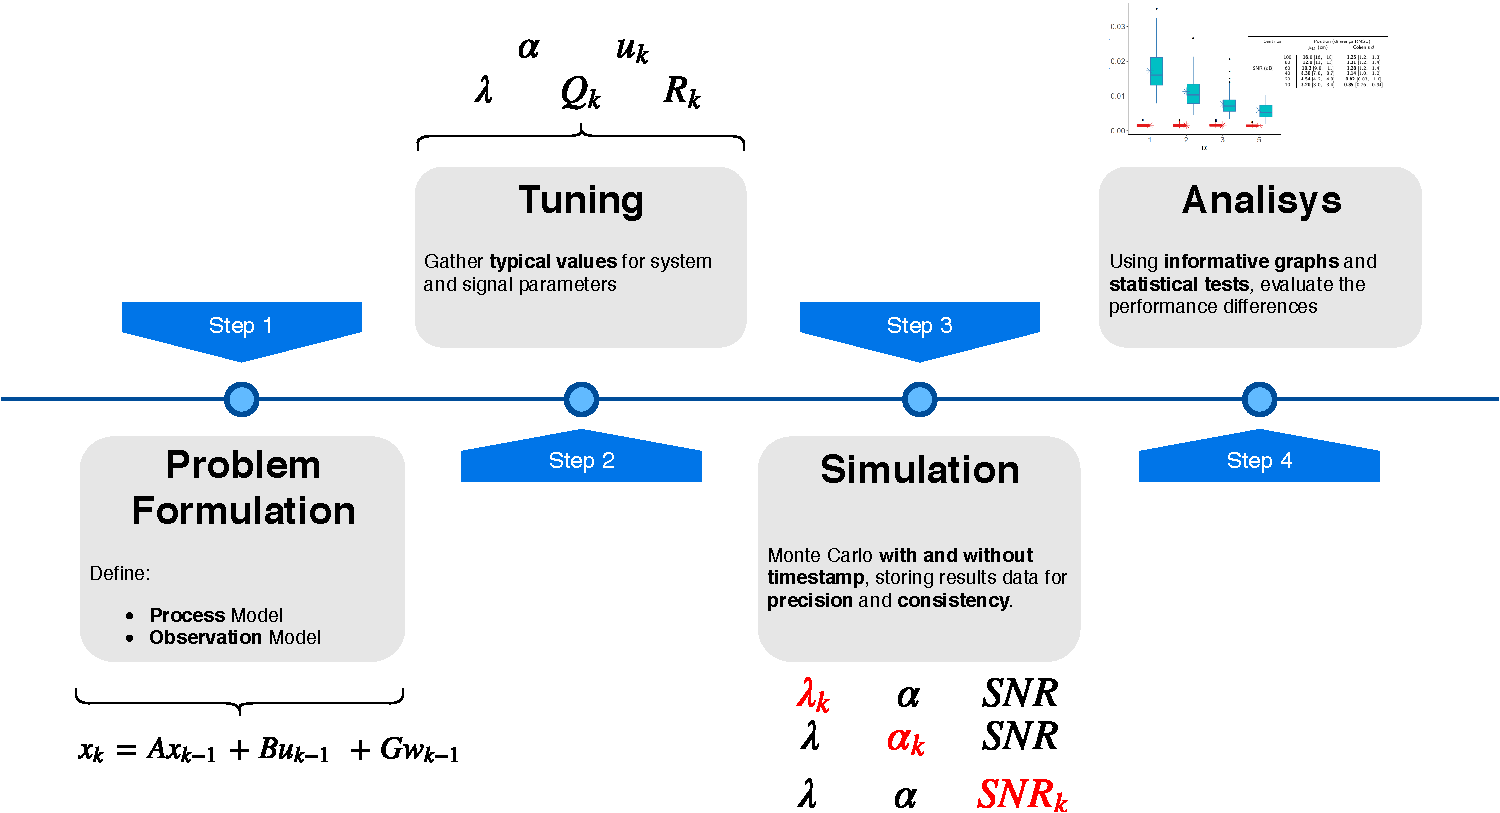
\includegraphics[width=1\textwidth]{Imagens/framework.pdf}
	%\setlength{\belowcaptionskip}{-12pt}
	\caption[Proposed framework]{Proposed framework steps to assist decision making process for investments in sensor networks and synchronization.}
	\label{fig:framework}
\end{figure} 

By applying the proposed framework to two different systems, one being linear and the other nonlinear, we test if the effects can indeed be assessed, fulfilling the last objective. For the case studies considered we observe some significant performance variation for some parameter sets, whereas for other combination of system parameters, neglecting timestamp did not play an important role. When system SNRs increase to a certain level, considering timestamp or not becomes irrelevant. Results suggest that timestamp information might algo be neglected for high sampling rates. However, what is considered to be high will depend on the system dynamics. Another conclusion we draw from results is that performance degradation for the variation of the relation between measurement and input sampling rates $\alpha$ might depend on the relation between their SNR levels. As a final note, we also observe a higher variability in performance metrics mean values for the algorithm that does not consider timestamp, which can be a problem if consistency is needed. Figure~\ref{fig:decision_flux} shows a suggestion of decision fluxogram, based on the proposed framework.

\begin{figure}[h]
	\centering
	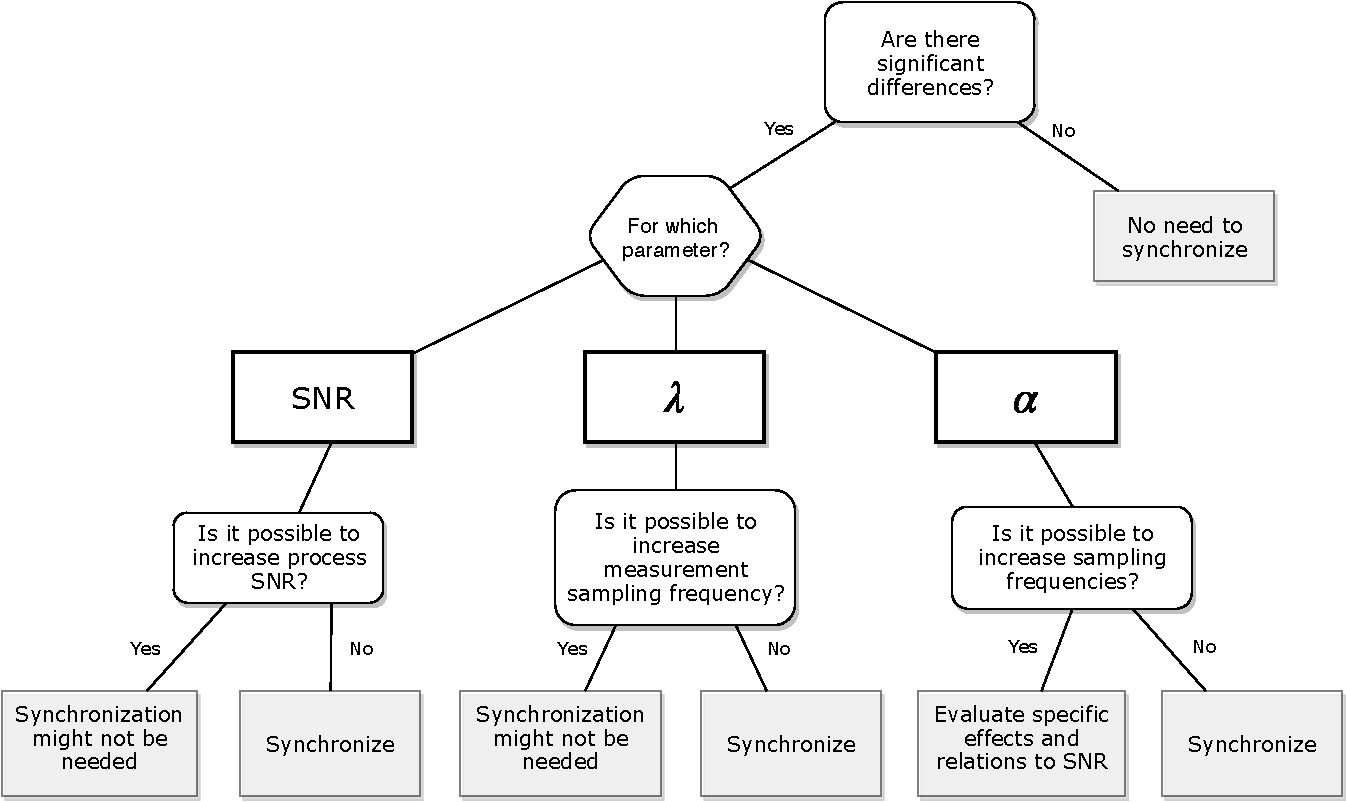
\includegraphics[width=1\textwidth]{Imagens/decision_flux.pdf}
	%\setlength{\belowcaptionskip}{-12pt}
	\caption[Proposed framework]{Proposed framework steps to assist decision making process for investments in sensor networks and synchronization.}
	\label{fig:decision_flux}
\end{figure} 

We must also be self-critical and question what could have been more consistent or realistic in our study. First, the irregular sampling model, although generic, could have been closer to reality by including time delay on data transmission. Such configuration would better justify the lack of timestamp in the data packet. However, time delay in state estimation without timestamps seems to have a similar effect to the problem we formulated, which is a time shift in measurement time instants. Adaptations to the algorithms, on the other hand, are much more complex. Additionally, as we observe in the results for $\alpha$ variation, different combination of SNR in process and observation models could have been carried out to evaluate a joint contribution. And finally, since we argue that neglecting timestamp will introduce an error to the measurements, then we could have tested state estimation algorithms with an artificially higher covariance of the observation model. We could also have tried some error compensation method that is related to an estimate of the output derivative, since they are related.

\section{Future Work}

From the improvement points discussed on the last section and some insights provided by the results, we identified some opportunities for further investigation, which are summarized as follows:

\begin{enumerate}
	\item A very clear relation between the error and the derivative of the signal was identified, one being directly proportional to the opposite of the other. We suggest the investigation of an error compensation algorithm to be used in state estimation;
	\item After using the proposed framework in simulations, a tuning routine seems promising, increasing the trace of the covariance matrix of the measurement noise. Although we showed that the added error is not white Gaussian, better state estimation performance might be achieved;
	\item In this study we did not include time delay as part of the irregular sampling problem. In real applications where transmission delays are present, new aspects of the systems might impact the degradation in performance and we suggest further investigation;
	\item We considered only Kalman filter and its unscented variation as state estimation algorithms in this study. We suggest the use of particle filter based methods to investigate if it will provide similar results. We argue that, since they are more promising for non-Gaussian noise, they could be more robust for scenarios where the signal-dependent error, introduced by neglecting timestamp, is more relevant;
	\item Further investigation in the variation of $\alpha$ for different combinations of SNR in process and observation models might also be interesting.
\end{enumerate}


\clearpage
%\afterpage{\blankpage}/